\section{Week 1: Recap}
\subsection{Section 1; Fermi-energy \& DOS}
\begin{exercise}
Show the following relations between the electron density, $\rho$, and the Fermi wave vector $k_F$ in the case of a 1,2, and 3-dimensional electron gas.
\end{exercise}
\begin{solution}
We start be finding the number of occupied states by defining $\ket{FS}$ as the Fermi sea and $\hat{N}$ being the number operator:
\begin{equation}\label{eq:p1e1}
	N = \expval{\hat{N}}{FS} = \sum_{q=\uparrow,\downarrow} \dfrac{\Omega_n}{(2\pi)^n}\int_{-\infty}^{\infty}\mathrm{d}\textbf{k}\expval{\hat{N}}{FS}
\end{equation}
Where $\Omega_n$ denotes $L$, $A$, and $V$ for $n = 1,2,3$ corresponding to 1D, 2D, and 3D respectively, $\sigma$ sums over spin states and $\hat{n} = [1+\exp{-(\varepsilon-\varepsilon_f)/k_bT}]^{-1}$ is the Fermi-Dirac distribution. At $T = 0$ the Fermi-Dirac distribution takes the form of a heavy side function (Step-Function), $\theta(k_f-k)$. The sum in \eqref{eq:p1e1} simply gives a factor of two, and dividing by $\Omega_n$ we obtain the density $\rho_n$:
\begin{equation}
	\rho_n \dfrac{(2\pi)^n}{2} = \int_{-\infty}^{\infty}\mathrm{d}\textbf{k} O(k_f-k) = \int_{-k_f}^{k_f}\mathrm{d}\textbf{k}
\end{equation}
Evaluating the integrals with the appropriate Jacobian yields:
\begin{equation}
	\rho_n \dfrac{(2\pi)^n}{2} = \begin{cases}
		2 k_f & ,\,1D \; \mathrm{for} \;  n = 1 \\
		\pi k_f^2 & ,\,2D \; \mathrm{for} \; n = 2 \\
		(4/3) \pi k_f^3 & ,\,3D \; \mathrm{for} \; n = 3
	\end{cases}
	\quad \Rightarrow \quad \begin{cases}
		k_f = (\pi/2) \rho_n & ,\,1D \\
		k_f^2 = 2 \pi \rho_n & ,\,2D \\
		k_f^3 = 3 \pi^2\rho_n & ,\,3D
	\end{cases}
\end{equation}
\end{solution}
\begin{exercise}
Calculate and sketch the density of states per length, area, and volume, respectively.
\end{exercise}
\begin{solution}
The density of states $D(\varepsilon)$ is defined as $D(\varepsilon) \equiv \mathrm{d}N/\mathrm{d}\varepsilon$. Using the chain rule we may write:
\begin{equation}
	 D(\varepsilon) \equiv \dfrac{\mathrm{d}N}{\mathrm{d}\varepsilon} = \dfrac{\mathrm{d}N}{\mathrm{d}k}\dfrac{\mathrm{d}k}{\mathrm{d}\varepsilon} = \dfrac{\mathrm{d}N}{\mathrm{d}k} \dfrac{1}{\mathrm{d}\varepsilon/\mathrm{d}k} = \dfrac{\mathrm{d}N}{\mathrm{d}k} \dfrac{1}{k}
\end{equation}
where the last equality arises from the energy relation of the free electron gas with energy given by $\varepsilon = k^2\hbar^2/(2m) \Rightarrow k^2/2$ in atomic units, e.g. $\hbar = 1$, $m = 1$. \textbf{Note:} The inversion of the derivative in the above expression is not generally allowed, it is only allowed in this case as we are dealing with polynomials. \\
The derivative of $N$ can be found by:
\begin{equation}\label{eq:p1e5}
    N = \rho_n \Omega_n = \Omega_n\begin{cases}
        2k/\pi & ,\,1D \\
        k^2/(2\pi) & ,\,2D \\
        k^3/(3\pi^2) & ,\,3D \\
    \end{cases} \Rightarrow \dfrac{\mathrm{d}N}{\mathrm{d}\varepsilon} = \Omega_n \begin{cases}
        2/\pi & ,\,1D \\
        k/\pi & ,\,2D \\
        k^2/\pi^2 & ,\,3D \\
    \end{cases}
\end{equation}
Using $k = \sqrt{2\varepsilon}$, inserting in \eqref{eq:p1e5}, we obtain:
\begin{equation}
    D_{1\mathrm{D}}(\varepsilon) = \dfrac{L}{\pi}\sqrt{\dfrac{2}{\varepsilon}} \quad,\quad D_{2\mathrm{D}}(\varepsilon) = \dfrac{A}{\pi}\quad,\quad 
    D_{3\mathrm{D}}(\varepsilon) = \dfrac{V}{\pi^2}\sqrt{2\varepsilon}
\end{equation}
\begin{figure}
    \centering
    \begin{minipage}{0.33\textwidth}
        \begin{tikzpicture}
        	\begin{axis}[
        		xlabel=$D(\varepsilon)$,
        		ylabel={$\varepsilon$},
        		samples=300,
        		xmin=0,
        		xmax=pi,
        		ticks=none,
        		axis x line=bottom,
        		axis y line=left,
        		width = 1\textwidth
        	]
        	\node at (axis cs:  2.8, 3.6) {1D};
        	% use TeX as calculator:
        	\addplot+[name path=f,color=black,mark=none] {1/sqrt(x)};
        	\path[name path=axis] (axis cs:0,0) -- (axis cs:1,0);
        	\addplot [thick,color=black,fill=black,fill opacity=0.05] fill between[of=f and axis];
        	\end{axis}
        \end{tikzpicture}
    \end{minipage}\begin{minipage}{0.33\textwidth}
        \begin{tikzpicture}
        	\begin{axis}[
        		xlabel=$D(\varepsilon)$,
        		ylabel={$\varepsilon$},
        		samples=300,
        		xmin=0,
        		xmax=pi,
        		ticks=none,
        		axis x line=bottom,
        		axis y line=left,
        		width = 1\textwidth
        	]
        	\node at (axis cs:  2.8,  0.7) {2D};
        	% use TeX as calculator:
        	\addplot +[name path=f,mark=none,color=black] coordinates {(2, -1) (2, 3)};
        	\path[name path=axis] (axis cs:0,-1) -- (axis cs:0,5);
        	\addplot [thick,color=black,fill=black,fill opacity=0.05] fill between[of=f and axis];
        	\end{axis}
        \end{tikzpicture}
    \end{minipage}\begin{minipage}{0.33\textwidth}
        \begin{tikzpicture}
        	\begin{axis}[
        		xlabel=$D(\varepsilon)$,
        		ylabel={$\varepsilon$},
        		samples=300,
        		xmin=0,
        		xmax=pi,
        		ticks=none,
        		axis x line=bottom,
        		axis y line=left,
        		width = 1\textwidth
        	]
        	\node at (axis cs:  2.8,  4.5) {3D};
        	% use TeX as calculator:
        	\addplot+[name path=f,color=black,mark=none] {x^2};
        	\path[name path=axis] (axis cs:0,0) -- (axis cs:0,10);
        	\addplot [thick,color=black,fill=black,fill opacity=0.05] fill between[of=f and axis];
        	\end{axis}
        \end{tikzpicture}
    \end{minipage}
    \label{fig:p1f1}
    \caption{Density of states (DOS) in 1D, 2D, and 3D for the free electron gas.}
\end{figure}
\end{solution}

\subsection{Section 2; 1D chain \& dimer}
In this section we deal with three cases of a 1D chain. The simple case with one atom per unit cell, then with two atoms per unit cell, and lastly with alternating lattice spacing. All cases are schematically illustrated in figure \ref{fig:1D_Chain}.
\begin{figure}[!ht]
    \centering
    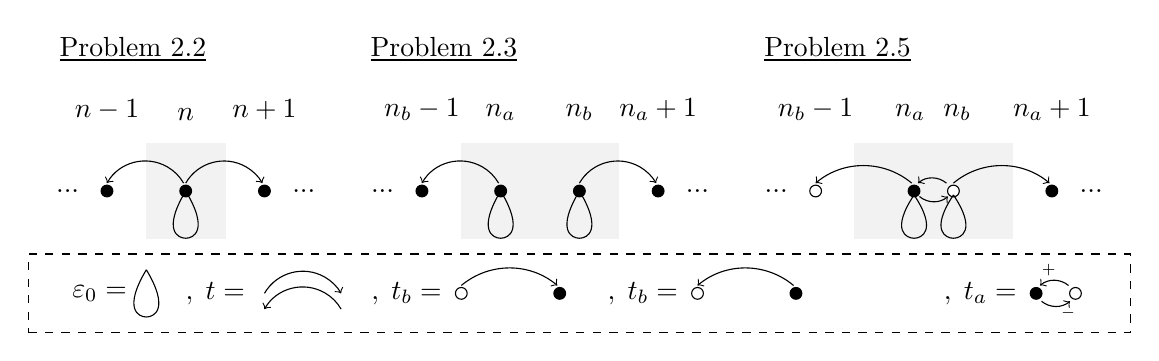
\begin{tikzpicture}[label distance = 0.7cm,
        mydot2/.style={circle, fill=white, draw, outer sep=0pt, inner sep=1.5pt},
        mydot1/.style={circle, fill=black, draw, outer sep=0pt, inner sep=1.5pt}]
        %%%%%%%%%% Label
            \node[label={[label distance = 0cm]east:{\underline{Problem 2.2}}}] at (-0.85,1.8) {};
            \node[label={[label distance = 0cm]east:{\underline{Problem 2.3}}}] at (3.1,1.8) {};
            \node[label={[label distance = 0cm]east:{\underline{Problem 2.5}}}] at (8.1,1.8) {};
        
        
        %%%%%%%%%% Legend
            \draw[dashed] (-1,-1.8) -| (13,-0.8) -| (-1,-1.8);
            
            % Epsilon
            \draw (0.5,-1) .. controls (0.2,-1.5) and (0.4,-1.6).. (0.5,-1.6)
                    (0.5,-1.6) .. controls (0.6,-1.6) and (0.8,-1.5) .. (0.5,-1);
            \node[label={[label distance = 0cm]west:{$\varepsilon_0 = $}}] at (0.5,-1.3) {};
        
            % T
            \draw [<-] (2,-1.5) arc (150:30:16pt); \draw [->] (2,-1.3) arc (150:30:16pt);
            \node[label={[label distance = 0cm]west:{$,\; t = $}}] at (2,-1.3) {};
            
            % Ta
            \draw [->] (4.5,-1.2) arc (130:50:27pt); \node[mydot2] at (4.5,-1.3) {}; \node[mydot1] at (5.75,-1.3) {};
            \node[label={[label distance = 0cm]west:{$,\; t_b = $}}] at (4.5,-1.3) {};
            
            % Tb
            \draw [<-] (7.5,-1.2) arc (130:50:27pt); \node[mydot2] at (7.5,-1.3) {}; \node[mydot1] at (8.75,-1.3) {};
            \node[label={[label distance = 0cm]west:{$,\; t_b = $}}] at (7.5,-1.3) {};
            
            % Ta - Tb
            \node[mydot1] at (11.8,-1.3) {}; \node[mydot2] at (12.3,-1.3) {};
            \draw [<-] (11.85,-1.2) arc (130:50:8pt); \draw [<-,rotate=180,shift={(-24.08,0.2)}] (11.85,1.2) arc (130:50:8pt);
            \node[label={[label distance = 0cm]west:{$,\; t_a = $}}] at (11.8,-1.3) {};
            \node[label={[label distance = 0cm]west:{\tiny{$+$}}}] at (12.3,-1) {};
            \node[label={[label distance = 0cm]west:{\tiny{$-$}}}] at (12.55,-1.55) {};
            
        
        %%%%%%%%%% problem 2.2
    	\node at (-0.5,0) {...}; \node at (2.5,0) {...};
    	\filldraw[fill=black!5!white, draw=black!5!white] (0.5,-0.6) rectangle (1.5,0.6);
    	\node[mydot1,label={above:{$\ket{n-1}$}}] (N11) at (0,0) {};
    	\node[mydot1,label={above:{$\ket{n}$}}] (N12) at (1,0) {};
    	\node[mydot1,label={above:{$\ket{n+1}$}}] (N13) at (2,0) {};
    	
        	%interaction
            \draw [<-] (0,0.1) arc (150:30:16pt); \draw [->] (1,0.1) arc (150:30:16pt);
            \draw (1,0) .. controls (0.7,-0.5) and (0.9,-0.6).. (1,-0.6)
                    (1,-0.6) .. controls (1.1,-0.6) and (1.3,-0.5) .. (1,0);
                
    	%%%%%%%%%% problem 2.3
    	\node at (3.5,0) {...}; \node at (7.5,0) {...};
    	\filldraw[fill=black!5!white, draw=black!5!white] (4.5,-0.6) rectangle (6.5,0.6);
    	\node[mydot1,label={above:{$\ket{n_b-1}$}}] (N21) at (4,0) {};
        \node[mydot1,label={above:{$\ket{n_a}$}}] (N22) at (5,0) {};
    	\node[mydot1,label={above:{$\ket{n_b}$}}] (N23) at (6,0) {};
    	\node[mydot1,label={above:{$\ket{n_a+1}$}}] (N24) at (7,0) {};

        	% interaction
        	\draw [<-] (4,0.1) arc (150:30:16pt); \draw [->] (6,0.1) arc (150:30:16pt);
            \draw (5,0) .. controls (4.7,-0.5) and (4.9,-0.6).. (5,-0.6)
                    (5,-0.6) .. controls (5.1,-0.6) and (5.3,-0.5) .. (5,0);
            \draw (6,0) .. controls (5.7,-0.5) and (5.9,-0.6).. (6,-0.6)
                    (6,-0.6) .. controls (6.1,-0.6) and (6.3,-0.5) .. (6,0);
                
    	%%%%%%%%%% problem 2.5
    	\node at (8.5,0) {...}; \node at (12.5,0) {...};
    	\filldraw[fill=black!5!white, draw=black!5!white] (9.5,-0.6) rectangle (11.5,0.6);
    	\node[mydot2,label={above:{$\ket{n_b-1}$}}] (N31) at (9,0) {};
    	\node[mydot1,label={above:{$\ket{n_a} \;$}}] (N32) at (10.25,0) {};
    	\node[mydot2,label={above:{$\; \ket{n_b}$}}] (N33) at (10.75,0) {};
    	\node[mydot1,label={above:{$\ket{n_a+1}$}}] (N34) at (12,0) {};

            % interaction
            \draw [<-] (9,0.1) arc (130:50:27pt); \draw [->] (10.75,0.1) arc (130:50:27pt);
            \draw [<-] (10.3,0.1) arc (130:50:8pt); \draw [<-,rotate=180,shift={(-20.98,-0.03)}] (10.3,0.1) arc (130:50:8pt);
            \draw (10.25,-0.05) .. controls (9.95,-0.5) and (10.15,-0.6).. (10.25,-0.6)
                    (10.25,-0.6) .. controls (10.35,-0.6) and (10.55,-0.5) .. (10.25,-0.05);
            \draw (10.75,-0.05) .. controls (10.45,-0.5) and (10.65,-0.6).. (10.75,-0.6)
                    (10.75,-0.6) .. controls (10.85,-0.6) and (11.05,-0.5) .. (10.75,-0.05);    
\end{tikzpicture}
    \caption{Schematic illustration of the orbitals, interactions, and numbering, of the 1D chains belonging to problem 2.2, 2.3, and 2.5.}
    \label{fig:1D_Chain}
\end{figure}

\begin{exercise}
show that the state 
\begin{equation}
    \ket{k} = \sum_{n = - \infty}^{\infty} e^{ikna} \ket{n}
    \label{eq:1.8}
\end{equation}
satisfies a discrete version of Bloch's theorem.
\end{exercise}

\begin{solution}
The approach is to take the inner product of the state with a projection $\bra{n+U}$, and show this is the same as $\braket{n}{k}$ up to a phase difference.
\begin{equation}
    \braket{n+U}{k} = \mel{n+U}{\sum_{n'=-\infty}^{\infty}e^{ikn'a}}{n'}
\end{equation}
This is only non-zero for $n'=n+U$, so
\begin{equation}
    \braket{n+U}{k} = \mel{n+U}{e^{ik(n+U)a}}{n+U} = e^{ik(n+U)a}\braket{n+U}{n+U} = e^{ikna}e^{ikUa}
\end{equation}
But from \eqref{eq:1.8} we have $\braket{n}{k} = e^{ikna}$, so the above reduces to
\begin{equation}
    \braket{n+U}{k} = \braket{n}{k}e^{ikUa}
\end{equation}
Thus it satisfies a discrete version of Bloch's theorem.


\end{solution}

\begin{exercise}
Calculate the band energies, $\varepsilon(k)$, for the wave vector $k$ in the first Brillouin zone, $k \in [-\frac{\pi}{a},\frac{\pi}{a}]$. Sketch the band structure and the density of states (DOS). Determine the center and width of the electronic band.
\end{exercise}
\begin{solution}
The band energies are found from
\begin{equation}
    \hat{H}\ket{k} = \varepsilon(k)\ket{k}
\end{equation}
So on applying the operator
\begin{equation}
    \hat{H}\ket{k} = \sum_n \varepsilon_0 c_n^{\dagger} c_n + t c_{n-1}^{\dagger} c_n + t c_{n+1}^{\dagger}c_n \sum_{n'} e^{ikn'a} \ket{n'}
\end{equation}
There will only be contributions from the 3 states $\ket{n'} = \ket{n} \text{ or } \ket{n \pm 1}$, so it reduces to
\begin{equation}
    \hat{H}\ket{k} = \sum_n \left[ \varepsilon_0 e^{ikna} + t e^{ik(n+1)a} + t e^{ik(n-1)a} \right] \ket{n} =  \left[ \varepsilon_0 + t e^{ika} + t e^{-ika} \right] \sum_n e^{ikna} \ket{n}
\end{equation}
According to equation \ref{eq:1.8}, and using that the complex exponentials in the square brackets can be written as 2 times cos this reduces to
\begin{equation}
   \varepsilon = \varepsilon_0 + 2 t \cos(ka) \ket{k}
   \label{eq:114}
\end{equation}

\begin{figure}
    \centering
    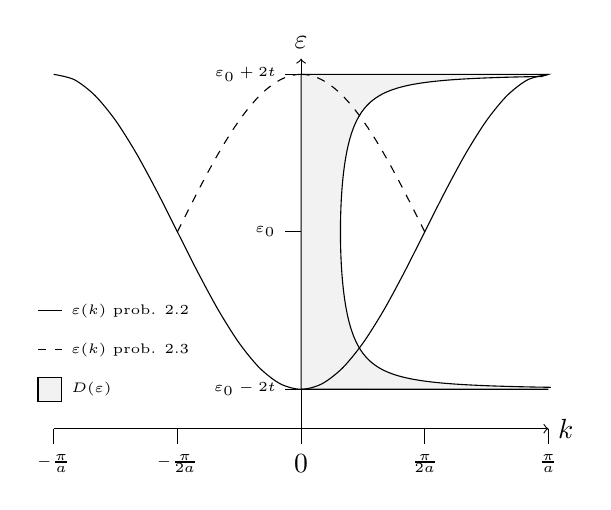
\begin{tikzpicture}
    % Axes
    \draw[->] (-pi,0) -- (pi,0) node[right] {$k$};
    \draw[->] (0,-0.2) -- (0,4.7) node[above] {$\varepsilon$};
    
    % Ticks
        %y
        \draw (0,4.5) -- (-0.2,4.5) node[left] {\tiny{$\varepsilon_0 + 2t$}};
        \draw (0,2.5) -- (-0.2,2.5) node[left] {\tiny{$\varepsilon_0$}};
        \draw (0,0.5) -- (-0.2,0.5) node[left] {\tiny{$\varepsilon_0 - 2t$}};
        
        %x
        \draw (-pi,0)   -- (-pi,-0.2)    node[below] {\tiny{$-\frac{\pi}{a}$}};
        \draw (-pi/2,0) -- (-pi/2,-0.2)  node[below] {\tiny{$-\frac{\pi}{2a}$}};
        \draw (0,0)     -- (-0,-0.2)     node[below] {$0$};
        \draw (pi/2,0)  -- (pi/2,-0.2)   node[below] {\tiny{$\frac{\pi}{2a}$}};
        \draw (pi,0)    -- (pi,-0.2)     node[below] {\tiny{$\frac{\pi}{a}$}};
    
    % Legend
    \draw (-pi-0.2,1.5) -- (-pi+0.1,1.5) node[right] {\tiny{$\varepsilon(k)$ prob. 2.2}};
    \draw[dashed] (-pi-0.2,1) -- (-pi+0.1,1) node[right] {\tiny{$\varepsilon(k)$  prob. 2.3}};
    \draw (-pi-0.2,0.5) -- (-pi+0.1,0.5) node[right] {\tiny{$D(\varepsilon)$}};
    \filldraw[fill=black!5!white] (-pi-0.2,0.35) rectangle (-pi+0.1,0.65);
    
    % DOS
    \filldraw[color=black,fill=black!5!white,smooth,samples=1000,variable=\y,domain=0.525:4.475] (0,0.5) -- (pi,0.5) plot ({(1/2)/(sqrt(1-(\y-2.5)*(\y-2.5)/4))},{\y}) --(pi,4.5) -- (0,4.5) -- (0,0.5);
    
    % Bands
    \draw[color=black,smooth,domain=-pi:pi]  plot (\x,{2.5-2*cos(\x r)});
    \draw[color=black,dashed,smooth,domain=-pi:(-pi/2)]  plot (\x+pi,{2.5-2*cos(\x r)});
    \draw[color=black,dashed,smooth,domain=(pi/2):pi]  plot (\x-pi,{2.5-2*cos(\x r)});
\end{tikzpicture}

    \caption{dispersion relation and DOS of the 1D chain in a 1 atom/unit cell (solid line) and 2 atoms/unit cell (dashed line).}
    \label{fig:1D_dispersion}
\end{figure}
    $\varepsilon(k) = \varepsilon_0 + 2 t \cos(ka)$ is sketched in figure \ref{fig:1D_dispersion}. 
    The density of states is found from isolating $k$ in $\varepsilon(k)$, and taking the derivative $D(\varepsilon) = \dv{k}{\varepsilon}$.
    \begin{equation}
        k(\varepsilon) = \frac{1}{a} \arccos\left(\frac{\varepsilon -\varepsilon_0}{2t} \right) \Rightarrow D(\varepsilon) = -\frac{1}{2ta} \frac{1}{\sqrt{1-\left(\frac{\epsilon-\epsilon_0}{2t} \right)^2}}
    \end{equation}
    The bandwidth is $4t$
\end{solution}

\begin{exercise}
Argue that the wave functions of the dimerized chain must have the form
\begin{equation}
    \ket{ks} = \sum_{n=-\infty}^{\infty} e^{ik(a+b)n} \left[ c_{as} \ket{n_a} + c_{bs} \ket{n_b} \right]
\end{equation}
\end{exercise}

\begin{solution}
It makes sense that the solution is found as a superposition of the states of the individual a and b states. No matter what these can serve as a basis for the solution.
$s=1,2$ as there will be two energy bands in this 2-state system.
\end{solution}

\begin{exercise}
Calculate the wave functions $\ket{sk}$ and band energies $\varepsilon_s(k)$. Sketch the
band structure and DOS of the dimerized chain, and determine the size of
the band gap, $E_{gap}$.
\end{exercise}

\begin{solution}
The system can be seen in the right most illustration in figure \ref{fig:1D_Chain}.
The Hamiltonian consists of 2 terms, that correspond to no jumping. Two terms of jumping within the unit cell, and two terms of jumping out of the cell, as illustrated in figure \ref{fig:1D_Chain}. Thus it is
\begin{equation}
    \hat{H} = \varepsilon_0 c_{na}^{\dagger}c_{na} + \varepsilon_0 c_{nb}^{\dagger}c_{nb} + t_a (c_{na}^{\dagger} c_{nb} + c_{nb}^{\dagger} c_{na} ) + t_b (  c_{(n-1)b}^{\dagger} c_{na} + c_{(n+1)a}^{\dagger} c_{nb})
\end{equation}
Where $t_a$ is the energy associated with jumping within the unit cell, and $t_b$ is associated with jumping out of the unit cell. \\
This system is put in matrix form in the $\ket{a}$ and $\ket{b}$ basis, and the eigenvalues and eigenfunctions will be found from diagonalising.
\begin{equation}
    \hat{H}_{ab} =
    \begin{bmatrix}
    \mel{a}{H}{a} & \mel{a}{H}{b} \\
    \mel{b}{H}{a} & \mel{b}{H}{b}
    \end{bmatrix}
\end{equation}
The diagonal terms only get contributions from the non-hopping elements. The off diagonal terms get contributions from hopping terms that go outside the unit cell, in this case a phase factor is multiplied on, applying Bloch's theorem.
\begin{equation}
    \hat{H}_{ab} =
    \begin{bmatrix}
    \varepsilon_0 & t_a + t_b e^{-ik(a+b)} \\
    t_a + t_b e^{ik(a+b)} & \varepsilon_0
    \end{bmatrix}
\end{equation}
Thus the energies are
\begin{equation}
\begin{split}
    (\varepsilon_0 - \lambda)^2 - (t_a + t_b e^{-ik(a+b)})(t_b + t_a e^{ik(a+b)}) = 0 \\ = (\varepsilon_0 - \lambda)^2 - (t_a^2 + t_b^2 + t_a t_b (e^{ik(a+b)} + e^{-ik(a+b)})) \\ = (\varepsilon_0 - \lambda)^2 - t_a^2 - t_b^2 - 2 t_a t_b \cos(k(a+b)) \\
    \Rightarrow \lambda =  \varepsilon_0 \mp \sqrt{ t_a^2 + t_b^2 + 2 t_a t_b \cos(k(a+b))}
\end{split}
\end{equation}



\begin{figure}
    \centering
    \begin{tikzpicture}
    % Axes
    \draw[->] (-pi,0) -- (pi,0) node[right] {$k$};
    \draw[->] (0,-0.2) -- (0,4.7) node[above] {$\varepsilon$};
    
    % Ticks
        %y
        \draw (-0.3,4.5)  (-0.5,4.5) node[left] {\tiny{$\varepsilon_0 + ta + tb$}};
        \draw (0,2.5) -- (-0.2,2.5) node[left] {\tiny{$\varepsilon_0$}};
        \draw (-0.3,0.5)  (-0.5,0.5) node[left] {\tiny{$\varepsilon_0 - ta - tb$}};
        
        %x
        \draw (-pi,0)   -- (-pi,-0.2)    node[below] {\tiny{$-\frac{\pi}{a}$}};
        \draw (-pi/2,0) -- (-pi/2,-0.2)  node[below] {\tiny{$-\frac{\pi}{2a}$}};
        \draw (0,0)     -- (-0,-0.2)     node[below] {$0$};
        \draw (pi/2,0)  -- (pi/2,-0.2)   node[below] {\tiny{$\frac{\pi}{2a}$}};
        \draw (pi,0)    -- (pi,-0.2)     node[below] {\tiny{$\frac{\pi}{a}$}};
    
    % Legend
    %\draw (-pi-0.2,1) -- (-pi+0.1,1) node[right] {\tiny{$\varepsilon(k)$}};
    %\draw (-pi-0.2,0.5) -- (-pi+0.1,0.5) node[right] %{\tiny{$D(\varepsilon)$}};
    %\filldraw[fill=black!5!white] (-pi-0.2,0.35) rectangle %(-pi+0.1,0.65);
    
    % DOS
    
    % Bands, ta=2/3, tb = 4/3, epsilon=2.5
    \draw[color=black,smooth,domain=-pi:pi]  plot (\x,{2.5-sqrt(4/9+16/9+16/9*cos(\x r))});
    \draw[color=black,smooth,domain=-pi:pi]  plot (\x,{2.5+sqrt(4/9+16/9+16/9*cos(\x r))});
\end{tikzpicture}

    \caption{dispersion relation and DOS of the 1D dimerised chain. Recalling that the short and long latice spacing, $a'$ and $b$ respectively, satisfy $a'+b = 2a$ where $a$ is the latice spacing of the non-dimerized chain.}
    \label{fig:1D_Dimer}
\end{figure}
It is seen that the energy of the lower band is lower in the dimerised case. This would imply that dimerisation is energetically favourable. However, the Coulomb energy is not taken into account in this model, and therefor there will be a competing term trying to create equal spacing. 
\end{solution}


\subsection{Section 3; Intuition on band structure}
\begin{exercise}
Sketch the band structure and the density of states (DOS) of: (A) an alkali
metal, (B) a noble metal, early (C) and late (D) transition metal, direct (E) and indirect (F) semi-conductor, and semi-metal (G) and graphene (H). 
\end{exercise}

\begin{solution}
TABLE of characteristics. \\
FIGURES comming up.
\end{solution}

